% !TeX root = ../main.tex
% Add the above to each chapter to make compiling the PDF easier in some editors.

\chapter{Convex Geometry}

We want to develop a better understanding of optimization problems. The general form of an \emph{optimization problem}\index{optimization problem} is, \begin{align}
    \min_{\substack{\vx \in \R^n \\ g_1(\vx) \leq b_1 \\ \vdots \\ g_m(\vx) \leq b_m}} f(\vx),
\end{align} where $f : \R^n \to \R$ and $g_i : \R^n \to \R$.\footnote{It suffices to consider minimization problems. If we want to maximize a function $f$, this is equivalent to minimizing the function $-f$.}

\begin{defn}[Feasible set] We call \begin{align}
    \spa{F} \defeq \{\vx \in \R^n \mid \forall i \in [n]: g_i(\vx) \leq b_i\}
\end{align} the \emph{feasible set}\index{feasible set}. We call \begin{itemize}
    \item $\vx \in \spa{F}$ a \emph{feasible point}\index{feasible point}; and
    \item $\vx \not\in \spa{F}$ an \emph{infeasible point}\index{infeasible point}.
\end{itemize}
\end{defn}
\begin{defn}[Optimal solution] We say that $\s{\vx} \in \R^n$ is \emph{optimal}\index{opimal point} if $\s{\vx} \in \spa{F}$ and $\forall \vx \in \spa{F}: f(\s{\vx}) \leq f(\vx)$.
\end{defn}
\begin{marginfigure}
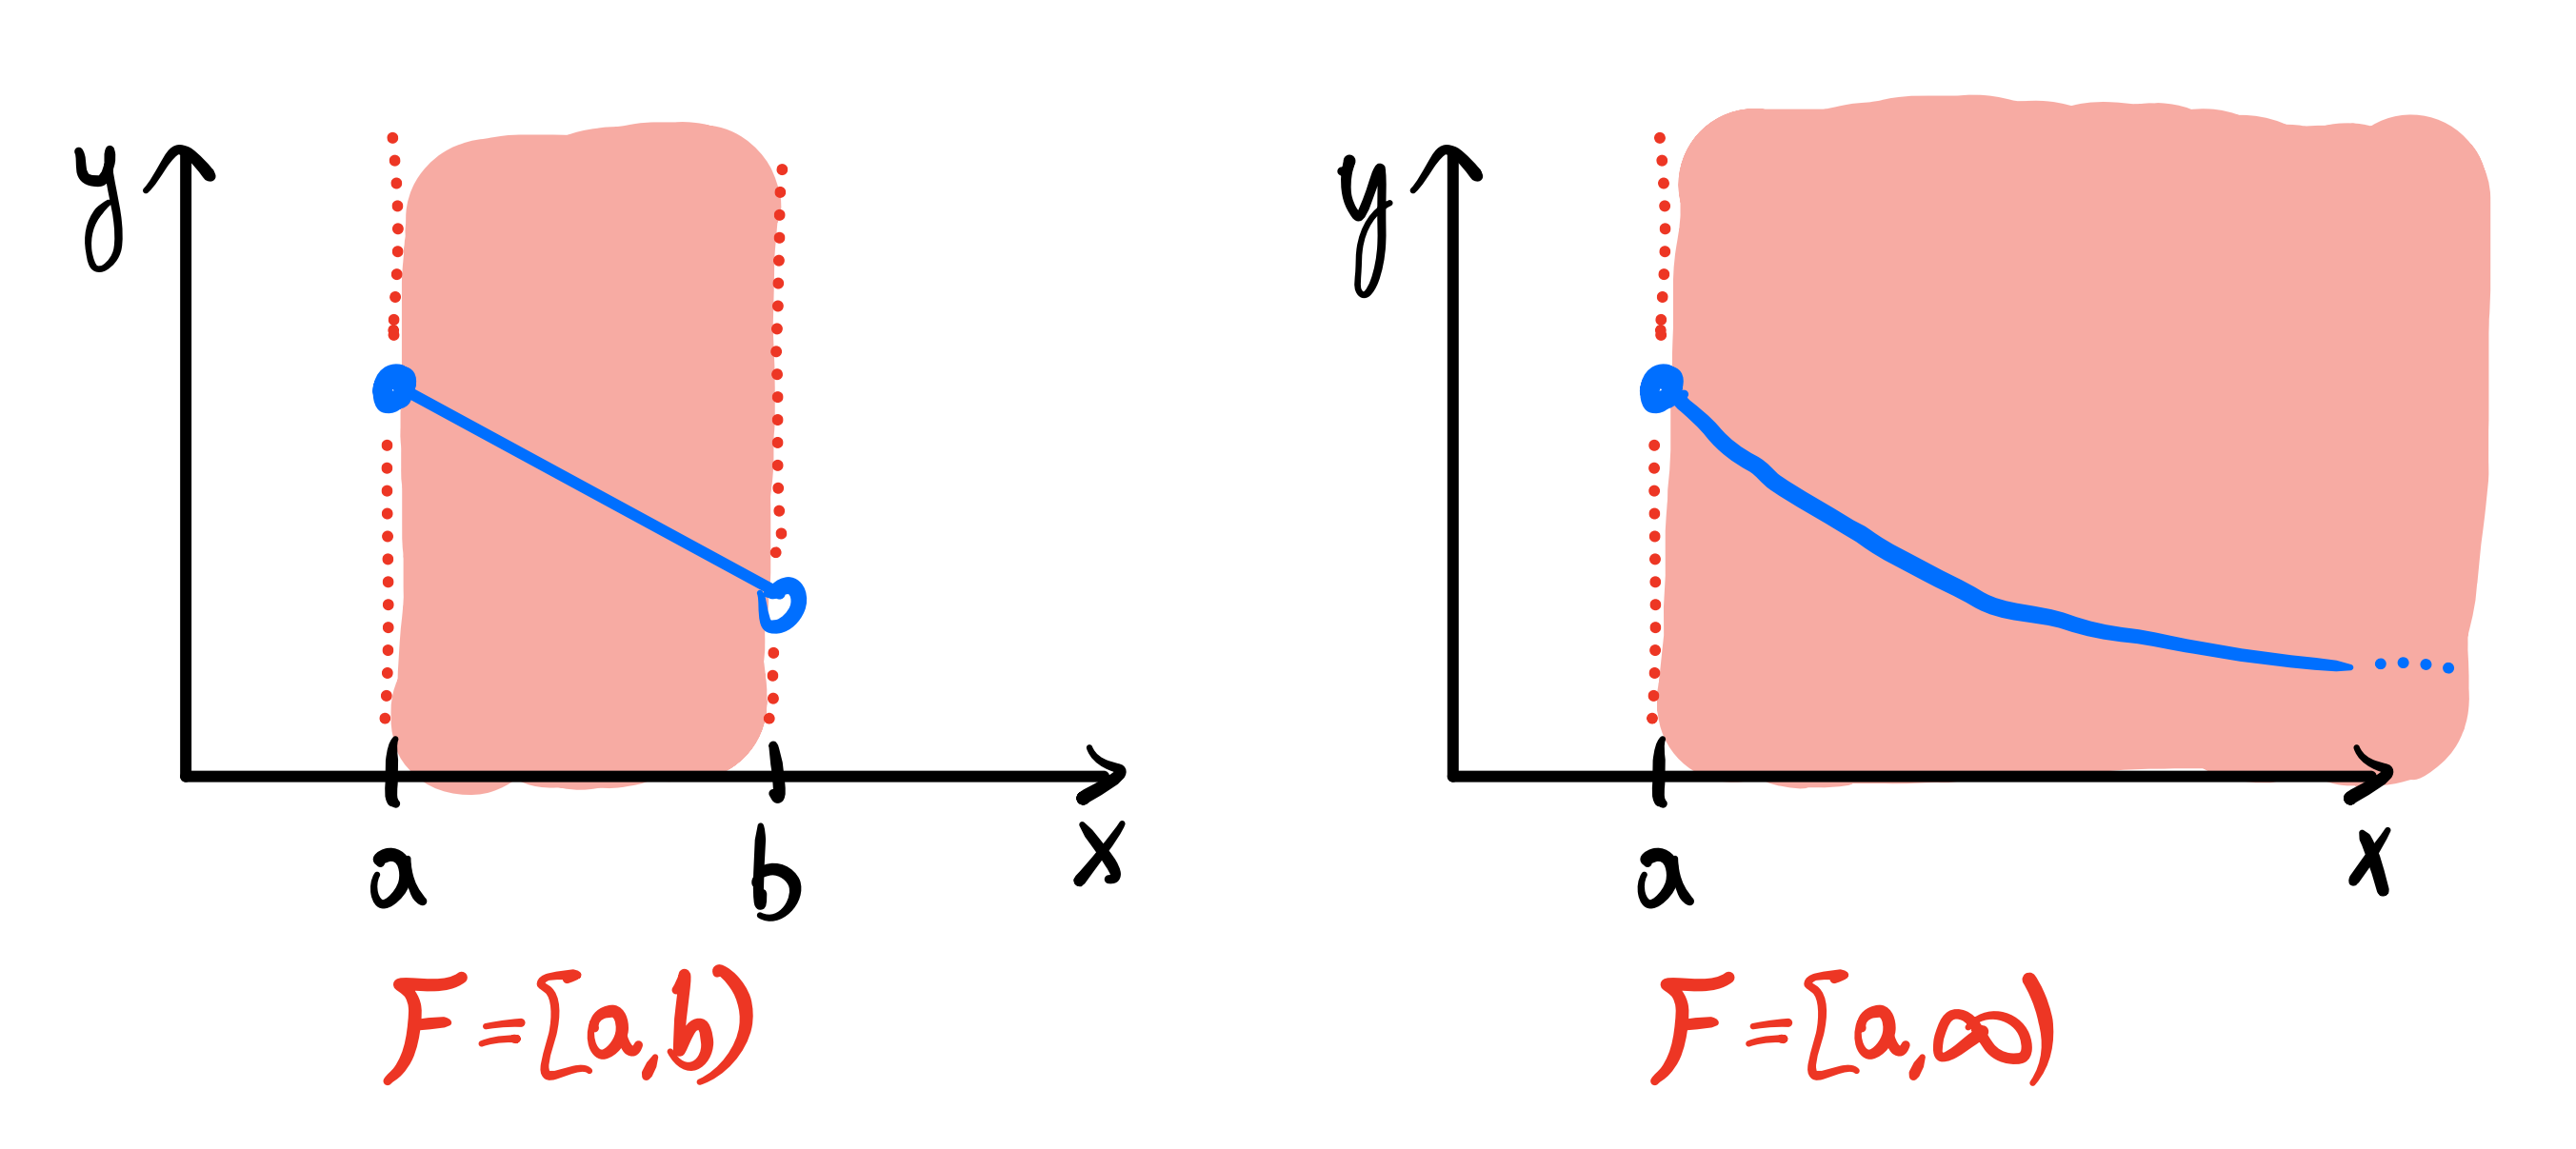
\includegraphics[width=\textwidth]{notes/figures/no_opt.png}
\caption{Examples of optimization problems without an optimal solution.}
\end{marginfigure}

Let us look at a sufficient condition for optimal solutions. \begin{thm}[Extreme value theorem]\index{extreme value theorem}
Let $f : \R^n \to \R$ be continuous, and let $\spa{F} \subseteq \R^n$ be non-empty, bounded, and closed. Then, $f$ is bounded on $\spa{F}$ and has an optimal solution.
\end{thm}

\section{Convex Sets \& Functions}

\begin{defn}[Convex set] A set $\sS \subseteq \R^n$ is \emph{convex}\index{convex set} iff \begin{align}
    \forall \vx, \vy \in \sS: \forall \theta \in [0,1]: \theta\vx + (1-\theta)\vy \in \sS.
\end{align}
\end{defn}
\begin{marginfigure}
\centering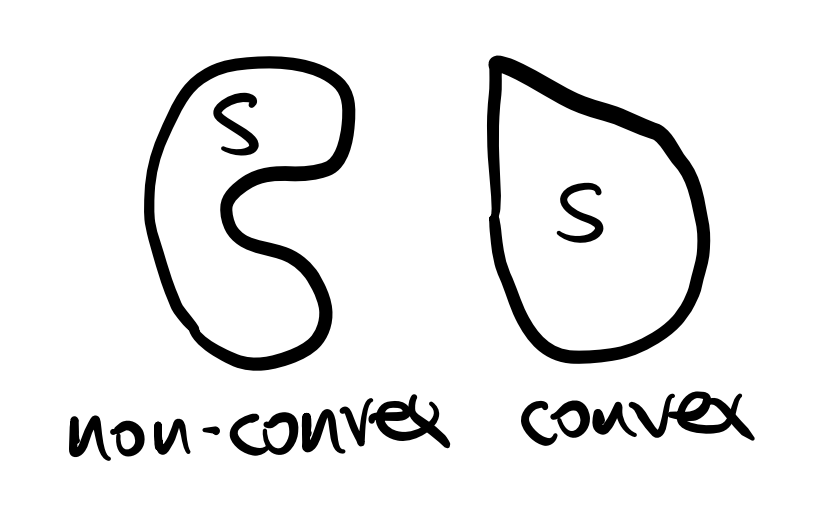
\includegraphics[width=4cm]{notes/figures/convex_set.png}
\caption{Example of a non-convex and a convex set.}
\end{marginfigure}
\begin{defn}[Convex function] For a convex set $\sS \subseteq \R^n$, a function $f : \sS \to \R$ is \emph{convex}\index{convex function} on $\sS$ iff \begin{align}
    \forall \vx, \vy \in \sS: \forall \theta \in [0,1]: f(\theta\vx + (1-\theta)\vy) \leq \theta f(\vx) + (1-\theta) f(\vy).
\end{align}
\end{defn}
\begin{marginfigure}
\centering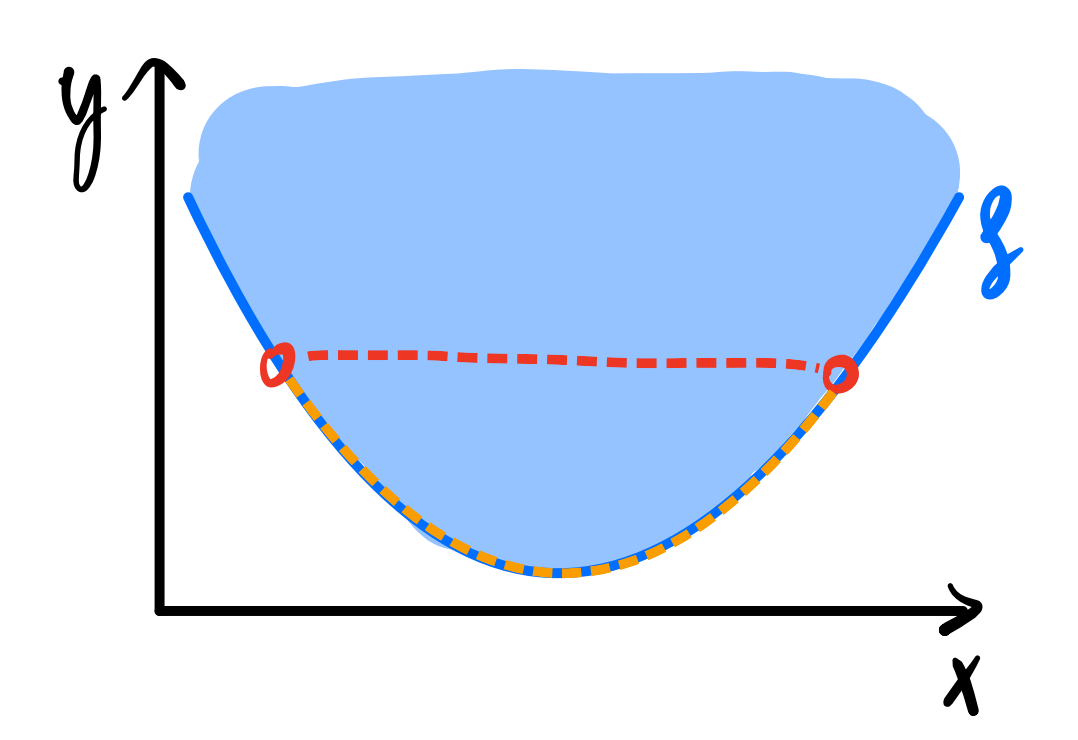
\includegraphics[width=3cm]{notes/figures/convex_function.png}
\caption{Example of a convex function. Any line between two points on $f$, lies ``above'' $f$. The epigraph of $f$ is shown in blue.}
\end{marginfigure}

\begin{rmk}
If the function $f$ is convex on $\sS$, we say that the function $-f$ is \emph{concave}\index{concave function} on $\sS$.
\end{rmk}

In the following, we will assume that $\sS \subseteq \R^n$ is open.

\begin{defn}[Epigraph]
The \emph{epigraph}\index{epigraph} of a function $f : \sS \to \R$ is \begin{align}
    \mathrm{epi}(f) \defeq \{(\vx,y) \mid f(\vx) \leq y\} \subseteq \R^{n+1}.
\end{align}
\end{defn}
\begin{lem}
The function $f : \sS \to \R$ is convex iff $\mathrm{epi}(f)$ is convex.\footnote{Proof in \cref{lem:b1}.}
\end{lem}

\begin{defn}[(Sub-)level set] Given a function $f : \sS \to \R$, we call, \begin{align}
    \sS_\alpha(f) &\defeq \{\vx \in \sS \mid f(\vx) \leq \alpha\}, \\
    \sL_\alpha(f) &\defeq \{\vx \in \sS \mid f(\vx) = \alpha\},
\end{align} its \emph{$\alpha$-sub-level set}\index{sub-level set} and \emph{$\alpha$-level set}\index{level set}, respectively.
\end{defn}
\begin{lem}
Any $\alpha$-sub-level set of a convex function is convex.\footnote{Proof in \cref{lem:b2}. Note that the other direction does not hold! Take $f(x) \defeq x^3$ as an example. Functions whose sub-level sets are convex are called \emph{quasiconvex}\index{quasiconvex}.}
\end{lem}

\section{First-order Characterization of Convexity}

\begin{marginfigure}
\centering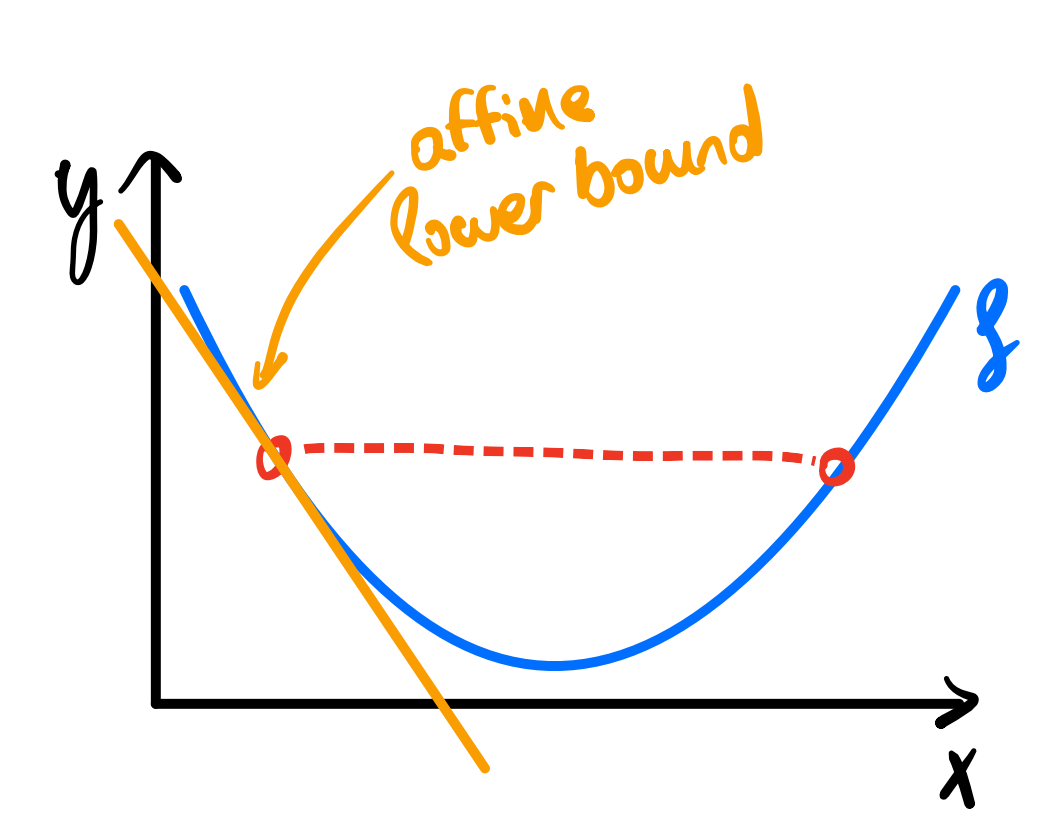
\includegraphics[width=3cm]{notes/figures/1st_order_characterization.png}
\caption{The first-order characterization characterizes convexity in terms of affine lower bounds.}
\end{marginfigure}
\begin{thm}[First-order characterization of convexity] Consider a differentiable function $f: \sS \to \R$. Then, $f$ is convex iff \begin{align}
    f(\vy) \geq f(\vx) + \trans{\grad f(\vx)}(\vy - \vx)
\end{align} for all $\vx, \vy \in \sS$.
\end{thm}
\begin{proof} \begin{itemize}
    \item ``$\Rightarrow$'': Fix any $\vx, \vy \in \sS$. As $f$ is convex, \begin{align*}
        f((1-\theta)\vx + \theta\vy) \leq (1-\theta)f(\vx) + \theta f(\vy),
    \end{align*} for all $\theta \in [0,1]$. We can rearrange to, \begin{align*}
        f(\underbrace{(1-\theta)\vx + \theta\vy}_{\vx + \theta(\vy - \vx)}) - f(\vy) \leq \theta(f(\vx) - f(\vy)).
    \end{align*} Dividing by $\theta$ yields, \begin{align*}
        \frac{f(\vx + \theta(\vy - \vx)) - f(\vx)}{\theta} \leq f(\vy) - f(\vx).
    \end{align*} Taking the limit $\theta \to 0$ on both sides gives the directional derivative at $\vx$ in direction $\vy - \vx$, \begin{align*}
        \trans{\grad f(\vx)}(\vy - \vx) = D f(\vx)[\vy - \vx] \leq f(\vy) - f(\vx).
    \end{align*}
    
    \item ``$\Leftarrow$'': Fix any $\vx, \vy \in \sS$ and let $\vz \defeq \theta\vy + (1-\theta)\vx$. We have, \begin{align*}
        f(\vy) &\geq f(\vz) + \trans{\grad f(\vz)}(\vy - \vz), \quad\text{and} \\
        f(\vx) &\geq f(\vz) + \trans{\grad f(\vz)}(\vx - \vz).
    \end{align*} We also have $(1-\theta)(\vy-\vx) = \vy - \vz$ and $\theta(\vy - \vx) = \vx - \vz$. Hence, \begin{align*}
        \theta f(\vy) + (1-\theta) f(\vx) &\geq f(\vz) + \trans{\grad f(\vz)}(\underbrace{\theta(\vy - \vz) + (1-\theta)(\vx - \vz)}_{0}) \\
        &= f(\theta\vy + (1-\theta)\vx). \qedhere
    \end{align*}
\end{itemize}
\end{proof}

\begin{thm} Let $f: \sS \to \R$ be a convex and differentiable function. Then, if $\vx \in \sS$ is a stationary point of $f$, then $\vx$ is a global minimum of $f$.
\end{thm}
\begin{proof} By the first-order characterization of convexity, we have for any $\vy \in \sS$, \begin{align*}
    f(\vy) \geq f(\vx) + \trans{\underbrace{\grad f(\vx)}_{0}}(\vy - \vx) = f(\vx). &\qedhere
\end{align*}
\end{proof}

\section{Second-order Characterization of Convexity}